%% LyX 2.0.6 created this file.  For more info, see http://www.lyx.org/.
%% Do not edit unless you really know what you are doing.
\documentclass[a4paper,american]{book}

\usepackage[turkish]{babel}
\usepackage[utf8]{inputenc}
\usepackage[T1]{fontenc}
%\usepackage[latin9]{inputenc}
\pagestyle{plain}
\setcounter{tocdepth}{3}
\synctex=-1
\usepackage{amssymb}
\usepackage{xkeyval}
\usepackage{graphicx}

\makeatletter

%%%%%%%%%%%%%%%%%%%%%%%%%%%%%% LyX specific LaTeX commands.
\pdfpageheight\paperheight
\pdfpagewidth\paperwidth

%% Because html converters don't know tabularnewline
\providecommand{\tabularnewline}{\\}

%%%%%%%%%%%%%%%%%%%%%%%%%%%%%% Textclass specific LaTeX commands.
\newenvironment{lyxcode}
{\par\begin{list}{}{
\setlength{\rightmargin}{\leftmargin}
\setlength{\listparindent}{0pt}% needed for AMS classes
\raggedright
\setlength{\itemsep}{0pt}
\setlength{\parsep}{0pt}
\normalfont\ttfamily}%
 \item[]}
{\end{list}}

%%%%%%%%%%%%%%%%%%%%%%%%%%%%%% User specified LaTeX commands.
\usepackage{wrapfig}
 \setlength{\intextsep}{0cm plus1cm minus1cm}
\newcommand{\menuitem}[1]{\textbf{\emph{#1}}}

\makeatother
\begin{document}
\shorthandoff{=}
\begin{flushleft}
\thispagestyle{empty}
\par\end{flushleft}

\vspace{0.2in}


\begin{center}
{\Huge{expEYES }}{\Large{Junior}}
\par\end{center}{\Large \par}

\begin{center}
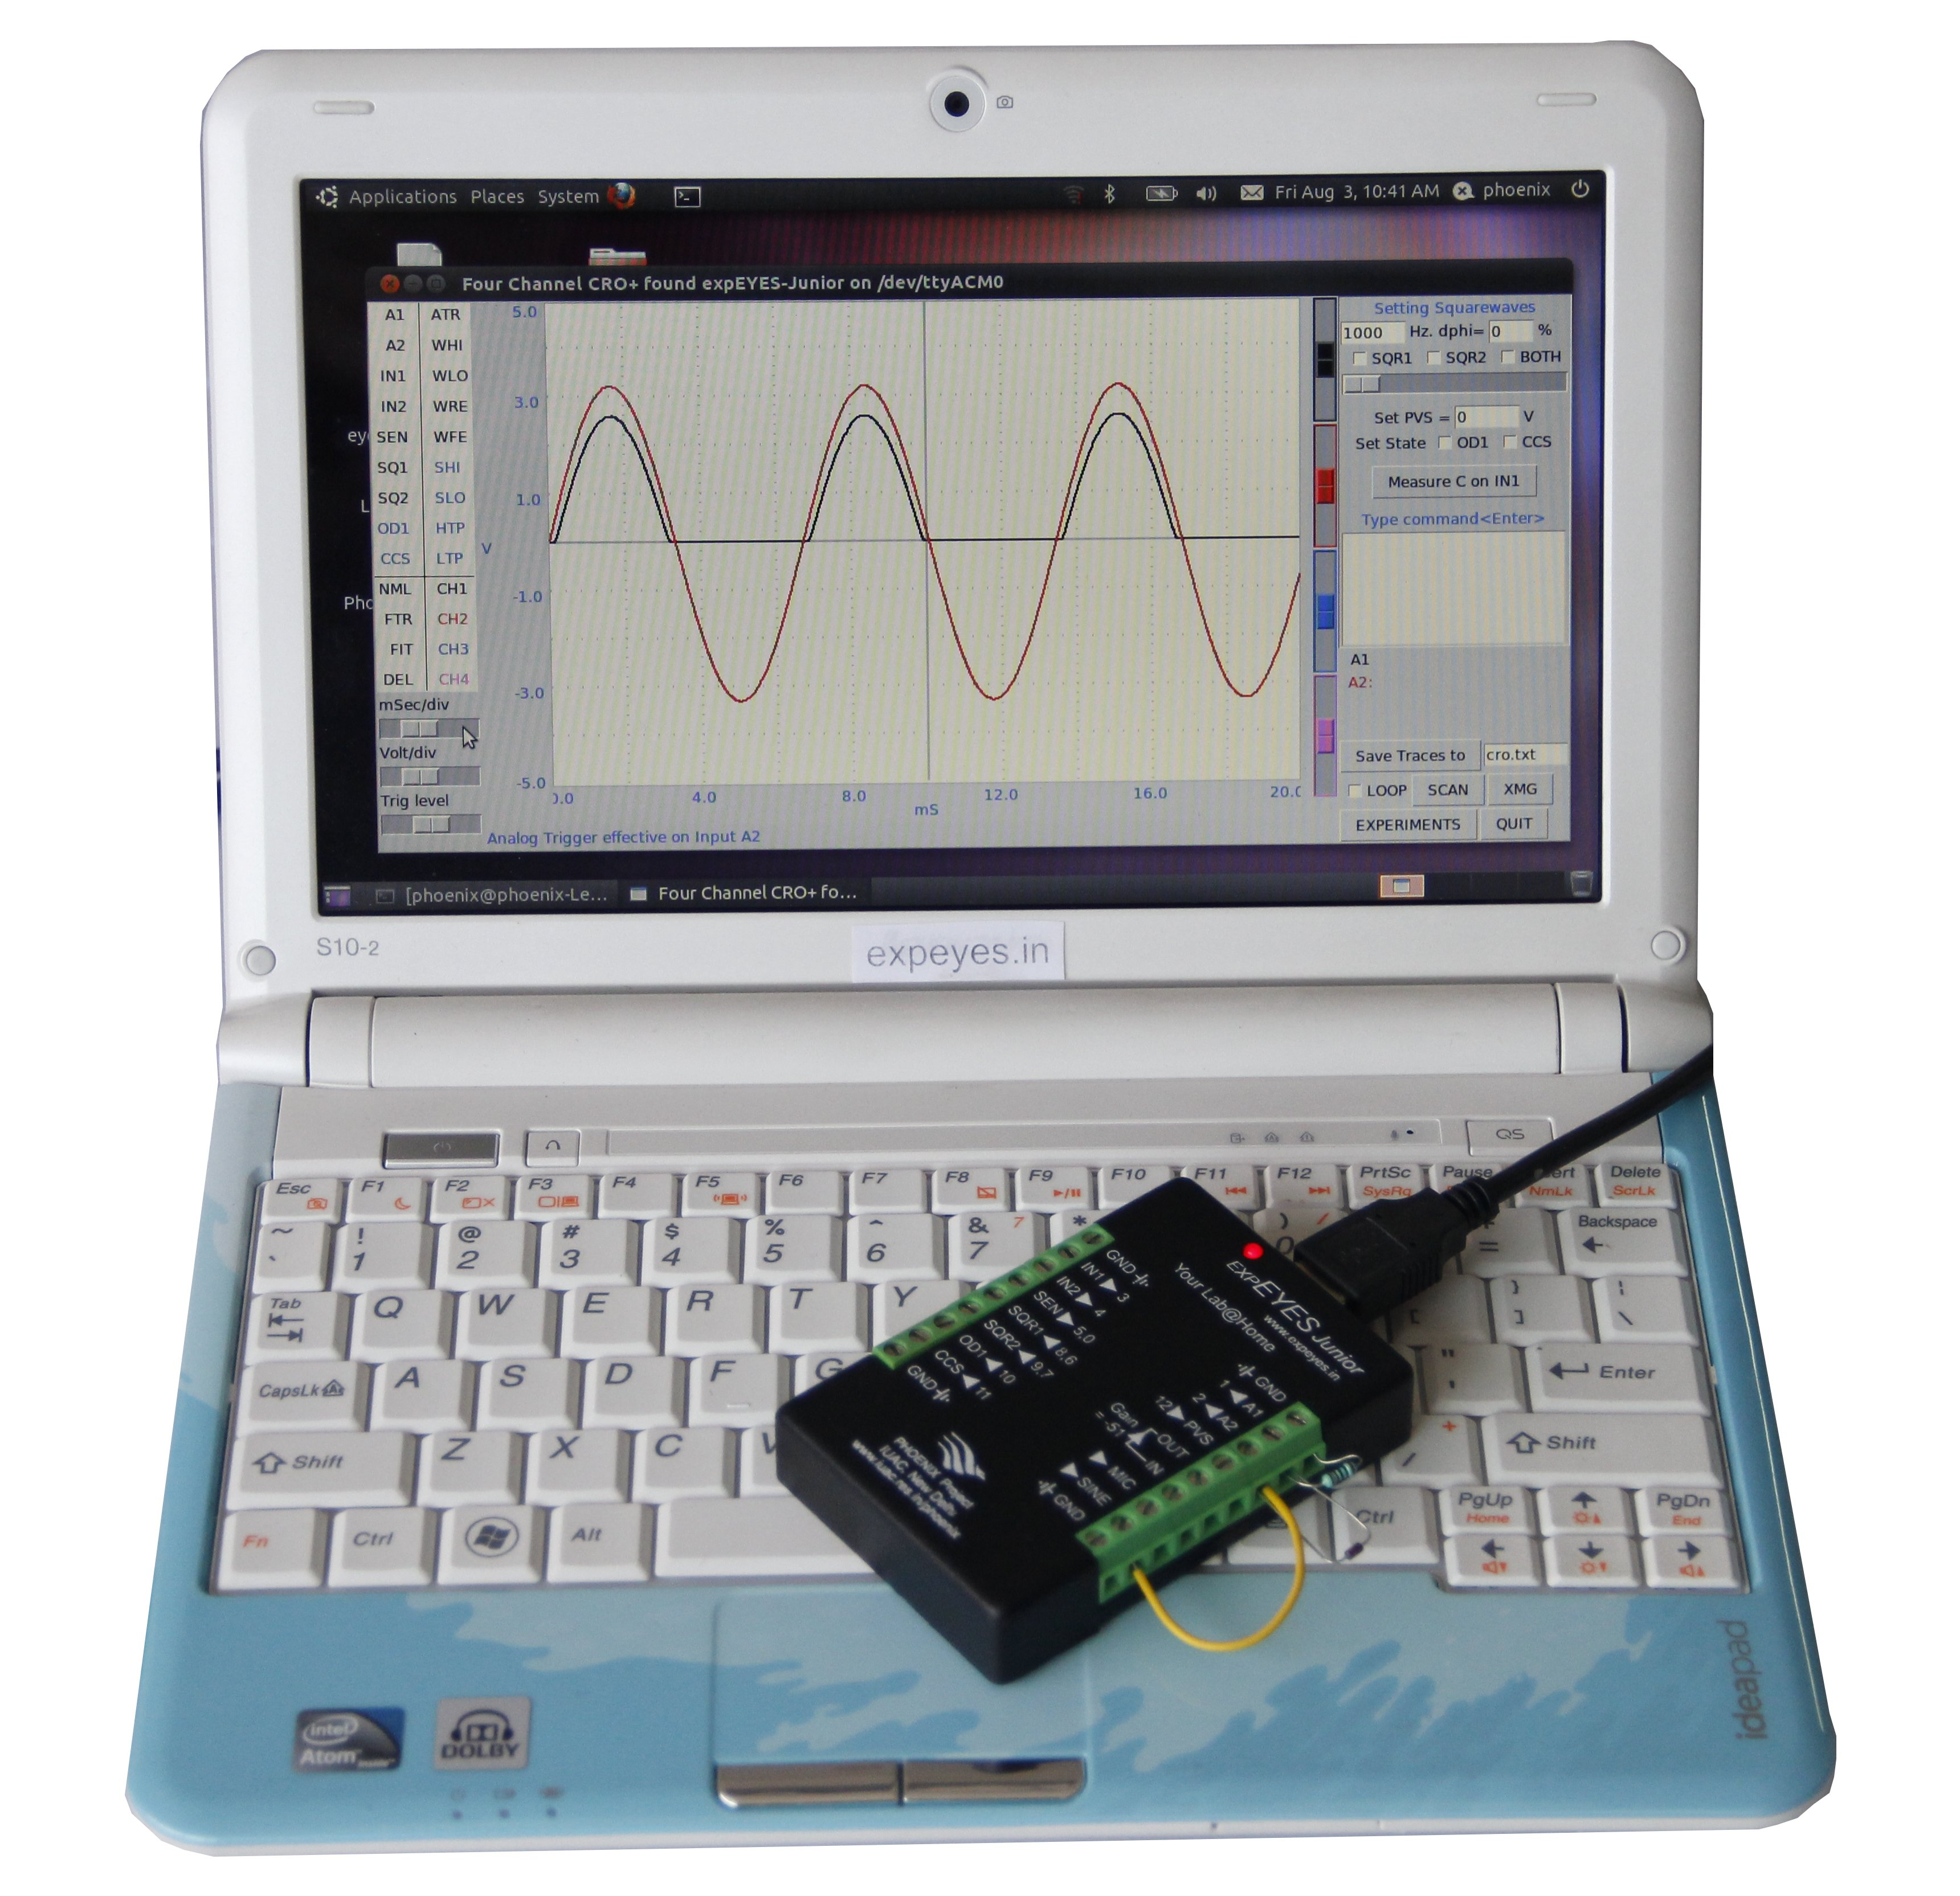
\includegraphics[width=5cm]{pics/ej-with-netbook-hr}
\par\end{center}

\begin{center}
{\large{User's Manual }}
\par\end{center}{\large \par}

\begin{center}
{\LARGE{Experiments for}}\\
{\LARGE{ Young Engineers and Scientists}}
\par\end{center}{\LARGE \par}

\begin{center}
http://expeyes.in
\par\end{center}

\begin{center}
from
\par\end{center}

\begin{center}
PHOENIX Project\\
Inter-University Accelerator Centre \\
(A Research Centre of UGC)\\
New Delhi 110 067\\
www.iuac.res.in
\par\end{center}

\newpage{}

Giriş

PHOENIX (Ev Yapımı Aletlerle Yenilikçi Deneyler) projesi
Hindistan Inter Üniversitesi Hızlandırıcı Merkezi tarafından 
Hindistan Üniversitelerindeki bilim eğitimini geliştirmek amacıyla 2004
yılında başlatılmıştır. Düşük bütçeli laboratuvar deney aleti geliştirmek ve
öğretmenleri eğitmek bu projenin iki temel amacıdır. 

expEYES Junior, daha önce tasarlanmış olan expEYES'ın değiştirilmiş
halidir. Bu alet, lise ve daha yüksek eğitim seviyesindeki sınıfların
keşfederek öğrenmesi için tasarlanmıştır. Bu aletin tasarlanırken; basit, her
ortama uyarlanabilen, dayanıklı ve düşük bütçeli olması çalışılmıştır.
Alet düşük bütçesi ile herkese hitap etmektedir. Öğrencilerin, duvarla kapalı olan ve zil çaldıktan sonra kapanan
laboratuvarın dışına çıkıp deneyleri gerçekleştirmesini umuyoruz. 

Alet donanımı açık kaynak koduna sahiptir. Yazılımı, GNU Genel Halk
Lisansına sahiptir. Bu aleti kullanan IUAC
dışındaki 
toplulukların ve birçok insanın katkısı bu projenin yol almasına neden
olmuştur. Bu belgedeki deneyleri birbirinden bağımsız olarak
gerçekleştirerek, hataların düzeltilmesinde yardımcı olan S Venkataramanan ve
Prof. R Nagarajan'a teşekkür ederiz. 

expEYES  Junior kullanım kılavuzu GNU Özgür Belge Lisansı altında
dağıtılmaktadır. Bu proje hakkında daha fazla bilgi için \textit{expeyes.in}
sayfasını ziyaret ediniz.

~

Ajith Kumar B.P. ~~~~~~~~~(ajith@iuac.res.in)

V V V Satyanarayana

Jimson Sacharias

\newpage{}

\tableofcontents{}


\chapter{Başlarken}


\section{Giriş}

Bilim, fiziksel dünyanın sistemli olarak gözlemlenmesi ve deneylerin
yapılmasıdır. Batıl inanç ve körü körüne inanmanın yerine mantıklı
düşünmenin oluşması için uygun bilim eğitimi gereklidir. Bilim eğitimi,
Teknikerlerin, mühendislerin ve bilim adamlarının eğitimi günümüz
dünyası ekonomisi için de gereklidir. Öğretmenler tarafından yapılan
gösteri deneyleri ya da öğrenciler tarafından gerçekleştirilen deneyler
pedagojik açıdan kişilerin deneyim kazanması açısından önemlidir. Fakat bilim
çoğunlukla deney yapılmadan çoğunlukla kitaplardan öğretilmektedir. Bunun
sonucunda, birçok öğrenci sınıfta elde ettiği deneyim ile günlük hayatta
karşılaştığı sorunlar arasında bağlantı kurmada başarısız olmaktadır. Bilim
eğitiminin keşif ve deney tabanlı olması ile bu bir ölçüde düzeltilebilir.

Kişisel bilgisayarların keşfi ve bunların kolay erişebilir olması,
laboratuvar deney aleti yapılması için yeni yollar açtı. Bilgisayarlara bazı
donanım eklenerek, bilgisayarlar bilim laboratuvarına çevrilebilir. Hızlı bir
şekilde deneylerin iyi bir doğrulukla yapılması, doğadaki birçok olayın
çalışılmasını mümkün kılar. Genelde bilim deneyleri, sıcaklık, basınç, hız,
voltaj, akım gibi değerlerin ölçülmesini ve kontrol edilmesini kapsar. Eğer
ölçülen fiziksel özellik hızlı bir şekilde değişiyorsa, ölçümlerin
otomasyonu sağlanmalıdır. Bilgisayar bu durumda faydalı bir alet olur.
Örneğin, AC'nin ( Değişken Akım) değişimini anlamak için mili saniyeler
aralıklarında ölçüm almak gerekir. 

Kabül edilebilir doğrulukla deneyleri gerçekleştirmek, araştırma temelli bilim
eğitiminin kapısını açar. Öğrenciler, elde ettikleri deneysel verileri
matematik modeller ile karşılaştırabilir ve çevremizdeki birçok doğal olayı
inceleyebilir. Bu, bilim araştırmacalarının daha karmaşık
aletlerle yaptıkları  deneylere benzerlik göstermektedir. expEYES(
expEriments for Young Engineers \& Scientists- Genç Bilim Adamları ve
Mühendisler için Deneyler) seti, okuldan üniversite sonrası eğitime kadar geniş
aralıktaki deneyleri desteklemek için tasarlanmıştır. Aynı zamanda
elektrik-elektronik mühendislerinin ve hobicilerin bunu test aleti olarak
kullanmasını sağlar. expEYES'in basit ve açık kaynak kodlu olması,
kullanıcıların \textit{detaya inmeden yeni deneyler geliştirmesine) olanak
verir.} Bu kullanıcı kılavuzu expEYES Junior'ı birkaç deney ile birlikte
açıklar. Bu kılavuza ek olarak, programcı kılavuzu da mevcuttur. 




\section{Donanım}

expEYES Junior, bilgisayarın USB portundan güç alır ve bu portu kullanarak
bilgisayar ile iletişime geçer. Dış sinyalleri bağlamak içinse, şekilde
gösterildiği gibi \ref{fig:The-ExpEYES-toppanel} her iki
tarafta birkaç tane
giriş/çıkış uçlarına sahiptir. expEYES, bu uçları kullanarak voltaj değişimlerini
izleyebilir ve kontrol edebilir. Diğer değişkenleri ( sıcaklık, basınç vb.)
ölçebilmek içinse, bunları uygun algılayıcılar kullanarak elektrik
sinyallerine çevirmek gerekir. 

Temel amacımız deney yapmak olsa bile, aşağıda verilen donanımın kısa bir
açıklamasını okumanız tavsiye edilir. Bu cihaz, elektrik-elektronik
mühendislik deneyleri için de kullanılabilir.  

\paragraph*{\textit{ÖNEMLİ : }}

\textit{expEYES'in uçlarına bağlanan voltaj değerleri izin verilebilen
değerler arasında olmalıdır. A1 ve A2 girişlerinin voltaj değerleri $\pm5$
voltaj aralığında; IN1 ve IN2 değerleri ise 0'dan 5V'a kadar olmalıdır. Bu
değerleri azıcık aşmak cihazın hata mesajı vermesine yol açacaktır. Eğer
program donarsa, USB kablosunu çıkarıp, yeniden takarak cihazı
başlatınız. Daha büyük voltaj değerleri ise cihaza kalıcı bir hasar
verecektir. Daha yüksek voltajları ölçmek için, potansiyel bölücü devre
kullanarak bu voltajları 5V'un altına düşürün. }

\begin{figure}
\begin{centering}
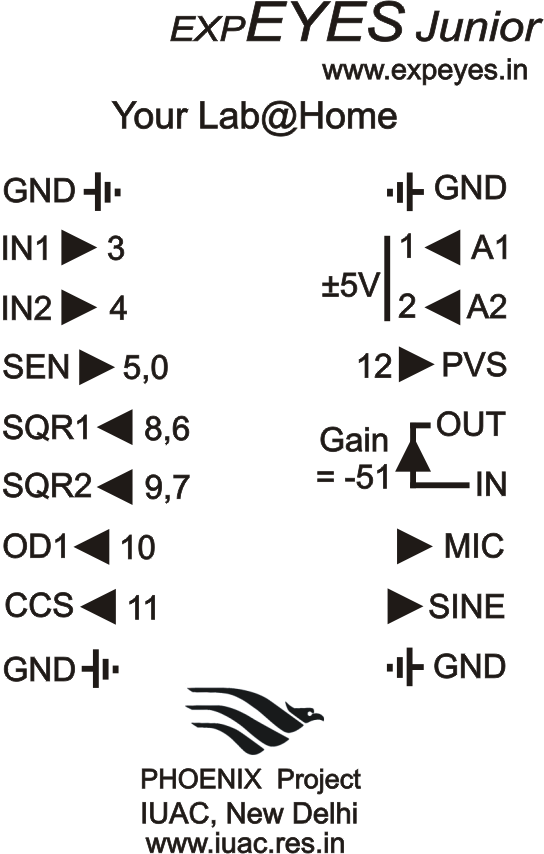
\includegraphics[height=9cm]{pics/top-panel}
\par\end{centering}

\caption{ExpEYES Junior'un üst yüzeyinin her iki tarafındaki
  bağlantılarının şekli. Bazı uçların üzerindeki numaralar, program
  yazarak bu uçlara erişmek isteyenler için verilmiştir. Oklar,
  sinyallerin yönünü göstermektedir. Örnek olarak $A1\Rightarrow1$ oku,
  A1 ucuna verilen sinyalin,  1 numaralı kanala gittiğini göstermektedir.  \label{fig:The-ExpEYES-toppanel}} 
\end{figure}



\subsection{Expeyes'in Uçları}

Giriş/Çıkış uçları kısaca aşağıda açıklanmıştır. 


\paragraph*{Programlanabilir Voltaj Kaynağı (PVS) :}

Bu ucun değeri, yazılım kullanarak 0 ile +5V arasında herhangi bir değere
ayarlanabilir. Bu voltajın çözünürlük değeri 12 bittir ve bu da her bir
voltaj değeri arasındaki değer farkının 1.25 milivolt'dan küçük
olamayacağını işaret eder. Bu uç tekrak okuma özelliği sayesinde PVS
değerini doğrular. 


\paragraph*{$\pm5V$ Analog Girişler (A1 \& A2) : }

Bu uçlar, $\pm5$ voltar aralığındaki voltaj değerlerini ölçebilir. Bu ucun ADC
(Analog Dijital Çevirici) değeri 12 bit'tir. Bu uçlardaki voltaj değerleri
zamana bağlı olarak bilgisayar ekranında gösterilebilir. Bu da cihazın düşük
frekansta osiloskop olarak kullanılmasını sağlar. Bu oskilloskopun en
yüksek örnekleme değeri saniyede 250,000 dir. Herbirinin giriş direnci
$10M\Omega$ dır. 

\paragraph*{$0-5V$ Analog Girişler (IN1 \& IN2):}

Bu uçlar 0 ile 5V arası voltaj değerlerini ölçebilir.


\paragraph*{Dirençsel Algılayıcı Girişi(SEN):}
Bu uç, Işık Orantılı Direnç, Isı Orantılı Direnç (Thermistor),
Foto-Transistör gibi algılayıcılar için tasarlanmıştır. SEN'in ucu
içindeki $5.1k\Omega$'lık direnci ile 5V'ta bağlanır. Bu uç aynı zamanda
gömülü analog karşılaştırıcıya sahiptir.


\paragraph*{Dijital Girişler (IN1 \& IN2):}

IN1 ve IN2 girişleri analog ve digital girişler olarak kullanılabilir.
Dijital giriş 


\paragraph*{Dijital Çıkış (OD1) :}

expEYES'in yazılımı kullanılarak OD1 Voltaj değeri 0 veya 5 volta
ayarlanabilir.

\paragraph*{Kare Dalga Üreticisi SQR1 \& SQR2 : }
Bu uçların çıkışları 0'dan 5 volta kadar değiştirilebilir. Frekans ise
0.7Hz'den 100kHz'e kadar ayarlanabilir. Bu aralık içindeki bütün frekans
değerleri mümkün değildir. SQR1 ve SQR2 birbirinden farklı frekans
değerlerine ayarlanabilir. Bunları birbirleriyle belli bir faz farkı olacak
şekilde aynı frekansa ayarlamak mümkündür. Bu çıkışlar, darbe genişliği
değişebilecek şekilde de programlanabilir. SQR1, geri okumalı olarak kanal
6'ya; SQR2 ise kanal 7'ye bağlanmıştır.

Frekansı $0$Hz'ye ayarlamak çıkışı yüksek (5V), $-1$'e ayarlamak ise çıkışı
düşük(0V) yapacaktır. Her iki durumda da dalga üretimi devredışı bırakılmış
olur. Bu iki çıkış devre dışı bırakıldığında, SQR1 ve SQR2, kanal 8 ve 9 için
dijital çıkıs olarak davranır. 

SQR1'in çıkışı \textbf{\textsl{ $100\Omega$ series resistor}} direnç
değerine sahiptir. Böylece bu çıkışa bağlanan bir LED'i direk olarak
çalıştırabilir. 



\paragraph*{Kızılötesi İletim}

SQR1'e bağlanacak bir kızılötesi (IR, infrared) diyot ile bu uç IR iletişim
sağlayabilir. 4 byte'lik iletişim ile bu uç bir TV kumandası gibi
davranabilir. Bu uç 1 byte'lik iletişimi de destekler. Bu iletişim 1
byte'lik iletişimi destekleyen mikroişlemciler tarafından alınabilir. \footnote{http://expeyes.in/micro-controllers-for-hobby-projects-and-education%
}.


\paragraph*{Sinüs Dalgası: }

Bu uç sabitlenmiş 150 Hz'lik frekans değerinde bir sinüs dalgası
üreticidir. Bu çıkış genliği 4V olan çift kutuplu(+4V,-4V) bir dalga üretir.


\paragraph*{Sabit Akım Üretici (CCS) : }

Sabit akım üreticisi, yazılım tarafından açılıp kapanabilir. Bu akımın
yaklaşık değeri 1mA dir, fakat bu değer elektronik parçalarındaki hata payı
yüzünden herbir cihazda farklılık gösterebilir. Bu akımın tam değerini
ölçmek için, CSS'den GND'ye bir akım ölçer takın. Diğer bir yöntem ise
değeri bilinen bir direnç (\textasciitilde{}3.3k) kullanarak, direnç
üzerindeki voltaj değerini ölçmektir. Bu direncin değeri 4k değerinden daha
düşük olması gereklidir. 
\paragraph*{Mikrofon (MIC) :}
Cihaz'ın yan tarafında, CCS'ye yakın dahili bir mikrofon vardır. 51 kere
yüksetilen bu çıkış, MIC çıkışına verilir. Bu çıkışı gözlemlemek için A1 veya
A2 uçları kullanılabilir.


\paragraph*{Ters Çevirici Yükseltici (IN->OUT) : }

Bu uç, ters çeviricili ( evirici ) yükselteç görevini görür. Yükselteç
(Op-Amp) olarak TL084 yongası (chip) kullanılmıştır. Rf = 51000 ve Ri =
1000, direnç değerleri kullanarak bu ucun en yüksek kazanç değeri
$\frac{51000}{1000}=51$ olarak bulunur. Bu değer giriş ucuna bir direnç
bağlanarak azaltılabilir. Örnek olarak bu girişin ucuna bağlanacak 50k'lık bir
direnç ile, kazancı $1$ olan bir tersleyici yükseltici yapılabilir.
\paragraph*{Ground : }

GND olarak işaretlenen uçlar toprak anlamına gelmektedir. Bütün ölçülen
voltajlar bu uçlara göre ölçülmektedir.


\subsection{Cihaz ile Birlikte Gelen Parçalar}

Bu cihaz ile birlikten gelen parçaların resmi bu kılavuzun arka kapağında
gösterilmiştir.
\begin{itemize}
\item Timsah ağızlı bağlantı kabloları (4) : Eğer uçlar arasındaki
  bağlantılar deney sırasında sıkça değiştirilirse, timsah ağızlı kabloları
  kullanarak bağlantılar kolayca yapılır.
\item 3000 Sarımlı Bobin (2) : 44SWG( 0.0813 cm yarıçaplı standart ölçüde
  kablo), İndüksiyon'u yaklaşık 125 mH, Direnci $\approx$ 500 $\Omega$. Bu
  bobinler indüksiyon, elektromanyetik indüksiyon, vb. çalışmalarında
  kullanılabilir. 
\item Piezo Elektrik Diskleri (Basınç duyarlı voltaj üreteçleri)  (2) :
  Rezonans frekansı yaklaşık 3500 Hz. dir. Bu disklere  SQR1 veya SQR2 ile
  enerji verilir. Diskler plastik bir kılıf içine yerleştirilmiştir. Bu
  kılıfın içinde oluşan
  oyuk, disk tarafından oluşturulan sesin genliğini arttırır. 
\item DC (Doğru Akım)  Motor : Bu motor 3 volt'dan daha az bir
  doğru akım gerilimle çalıştırılmalıdır.
\item Mıknatıs : (a) 10mm yarıçap \& uzunluğunda (b) 5 mm
  yarıçap \& 10 mm uzunluğunda
(c) Düğme boyutunda mıknatıs (2)
\item 5mm LEDS : KIRMIZI, MAVİ, YEŞİL, BEYAZ
\item Kapasitörler : 47uF, 1uF, 0.1uF \& 0.01 uF
\item Dirençler : 560$\Omega$, 1$k\Omega$, 2.2$k\Omega$ , 10$k\Omega$
, 51$k\Omega$ and 200 $k\Omega$
\item LDR(Işığa Duyarlı Direnç) \& Thermistor(Sıcaklığa Duyarlı Direnç) 
\item İki Silikon Diyot (1N4148) and 1 Transistor( 2N2222)
\item 5 tane 8cm uzunluğunda  
\end{itemize}

\section{Software Installation}

ExpEYES can run on any computer having a Python Interpreter and a
Python module to access the Serial port. The USB interface is handled
by the device driver program that presents the USB port as an RS232
port to the application programs. The communication the expEYES is
done using a library written in Python language (also available in
C language). Programs with GUI have been written for many experiments.
There are many ways to get the software running:


\subsubsection*{The expEYES Live CD }

The easiest way to get started is to boot your PC with the expEYES
Live-CD. From the PC BIOS, make the CD drive as the first boot device,
insert the live CD and reboot the PC. A desktop will appear and you
can start expEYES Junior from the menu \textbf{Applications->Science}->EYES-Junior.
You can also start it from a Terminal using the command:
\begin{lyxcode}
\$~python~/usr/share/expeyes-junior/croplus.py
\end{lyxcode}

\subsubsection*{Installing on Debian or Ubuntu GNU/Linux distributions}

Download \textbf{expeyes-3.0.0.deb} , or higher version, from the
software section of \textbf{http://expeyes.in} and install it. It
depends on python-serial, python-tk, python-scipy and grace (a 2D
plotting program).


\subsubsection*{For other GNU/Linux distributions}

Download \textbf{expeyes-3.x.x.zip} from \textbf{http://expeyes.in}
and follow the instructions in the README file. It is important to
give read/write permissions for all users on the USB port where expEYES
is connected. This can be done by running the \textit{postint} shell
script, included in the zip file.


\subsubsection*{On MSWindows}

Even though expEYES is Free Software and is developed using Free and
Open software, it runs on non-free platforms also. To install it on
MS windows, you need (1) MCP2200 drivers (2) Python-2.x version, python-serial,
python-tk, python-numpy and python-scipy (3) expeyes-3.x.x.zip

Unzip the file \textbf{expeyes-3.x.x.zip}, and double click on \textbf{croplus.py}
inside the newly created directory named expeyes-3.x.x\textbackslash{}eyes-junior.
If you have expEYES liveCD, browse inside the directory names WINEYES.
All the files mentioned above are inside that directory. Double click
on them in the order mentioned above to install them. See the software
section on the expeyes website for more details.


\section{The main GUI program}

\begin{figure}
\begin{centering}
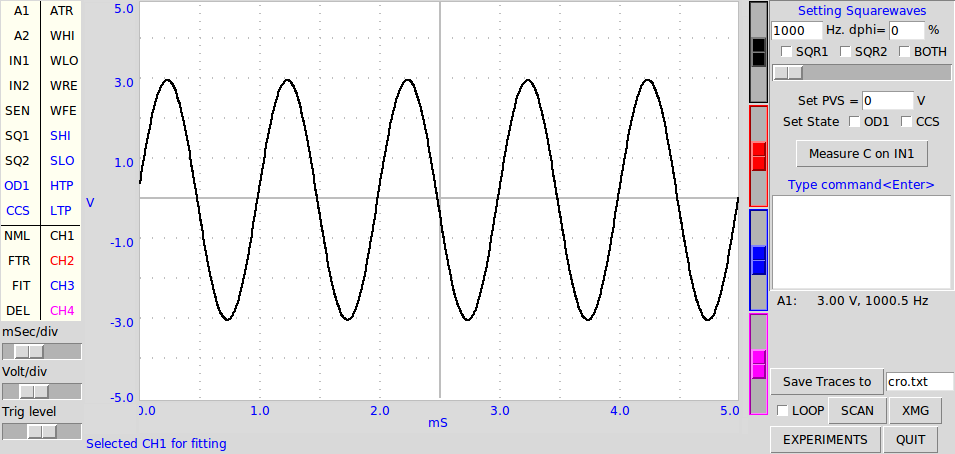
\includegraphics[width=11cm]{pics/benchmark}
\par\end{centering}

\caption{The croplus screen showing a sine-wave connected to A1. \label{fig:The-croplus-screen.}}
\end{figure}


Start Applications->Science->EYES-Junior from the menu. A four channel
oscilloscope screen with several extra features will open as shown
in figure \ref{fig:The-croplus-screen.}. The \textit{\menuitem{EXPERIMENTS}
}button pops up a menu of programs for several experiments. The main
window will become inactive when an experiment is selected and running.


\subsubsection*{The Plot Window}

The plot window works like a low frequency four channel oscilloscope.
The maximum sampling rate is 250 kHz only, sufficient for exploring
audio frequency range. A brief description of this GUI program is
given below.
\begin{itemize}
\item On the left side, the Inputs (A1,A2,IN1,IN2,SEN and read backs of
SQR1 \& SQR2) are shown. \textit{Clicking on any of them will display
the voltage/logic level present. }To plot any of them, drag it to
the desired channel (CH1 to CH4). The names of inputs selected for
display are shown on the right side of the plot window, using a unique
color for each channel.
\item For online help, place cursor on any item, press and hold the left
mouse button.
\item Dragging ATR to any of the inputs will make it the CRO trigger source.
\item This program allows different types of triggering. For example, dragging
WRE to IN1 will enable rising edge triggering on it. It also supports
setting levels or generating pulses on Digital outputs just before
capturing the waveform. Dragging SHI to OD1 will keep OD1 HIGH during
the capture process. For more details refer to the programmers manual.
\item Dragging any of the channels, CH1 to CH4, to FIT will enable calculating
amplitude and frequency by fitting the data using the equation $V=V_{0}\sin\left(2\pi ft+\theta\right)+C$
, $V_{0}$ and $f$ will be displayed. Dragging the channel to NML
will disable the FIT option.
\item Right clicking on IN1, IN2, SEN, SQR1 or SQR2 will measure the frequency
and duty cycle of the voltage waveform present at the terminal.
\item If two adjacent channels are assigned, Right-clicking on the first
will calculate frequency and phase difference between the two inputs.
\item Dragging a channel to FTR will show the Fourier Spectrum of the waveform
in a separate window.
\item To remove a displayed input, drag it to DEL.
\item Horizontal scale (ms/division) adjustment. Set this to the minimum
value and increase to view more number of cycles on the screen. Drag
the rider or click on the left/right sides of it.
\item Vertical scale (volts/division). Maximum values is 5 volts per division.
\item Vertical offset sliders are provided for each channel to shift the
trace up or down.
\item The Check button LOOP selects Single/Continuous mode of scanning.
\item The traces can be transferred to an Grace plot window, using XMG.
\item SAVE button to save the data to the specified file in\textit{ }two
column text format.
\end{itemize}
In addition to the CRO features, you can also control SQR1, SQR2,
PVS etc. from the GUI. You can execute Python functions to access
the hardware from a command window.
\begin{itemize}
\item For the Square waves , the frequency and phase difference in percentage
are entered in two text fields. SQR1 \& SQR2 can be set to different
frequencies or to a single frequency with desired phase difference.
Re-activate the check buttons after changing frequency or phase difference. 
\item SQR1 can be set using a slider also.
\item To Set PVS, type the voltage (0 to 5) and press Enter key. The PVS
output has a readback and the read back value is displayed in the
message field.
\item Checkbuttons are provided to control OD1 and CCS.
\item Capacitance connected between IN1 and GND can be measured.
\item Python functions to communicate to the hardware can be entered in
a Command Window.
\end{itemize}

\section{Basic measurements using expEYES}

Before proceeding with the experiments, let us do some simple exercises
to become familiar with expEYES Junior. Boot your computer from the
LiveCD, connect the device a USB port and start the EYES-Junior program
from the menu 'Applications->Science'.


\subsection{Generate \& measure voltages}
\begin{itemize}
\item Connect PVS to IN1 and Assign IN1 to CH1
\item Set PVS to some voltage and observe the trace
\item Click on IN1 to display the voltage.
\end{itemize}

\subsection{Observe voltage waveforms}
\begin{itemize}
\item Connect SINE to A1 and Assign A1 to CH1
\item Adjust the horizontal scale (ms/Div) to view 4 or 5 cycles of the
square wave
\item Set frequency to to 100 and Check SQR1.
\item Assign SQR1 to CH2
\item Change frequency. Uncheck and Check SQR1.
\item Explore the FIT and FTR options.
\end{itemize}

\subsection{Measure frequency \& Duty cycle}
\begin{itemize}
\item Set SQR1 to 1000
\item Right Click on SQR1 to display frequency and duty cycle.
\item To set 488 Hz 30\% PWM, enter \textit{set\_sqr1\_pwm(30)}%
\footnote{\textit{For information about all the commands, refer to the Programmer's
manual}%
}\textit{ }inside the Command window.
\item Measure again by Right Clicking on SQR1
\end{itemize}

\subsection{Accuracy and resolution}

Figure \ref{fig:The-croplus-screen.} shows a 3V, 3000.5 Hz sine wave
from an Agilent 33220A Function generator, connected to A1. The voltage
at IN1 is measured as 3.000 by a Keithley 2100 multimeter, off by
2mV. The frequency of audio frequency sine wave is measured with less
than 0.1\% error. The voltage measurement has 12 bit resolution but
the absolute accuracy may change slightly with ambient temperature.


\section{Experiments}

The expEYES hardware can generate/measure different kinds of voltage
signals. For measuring any other parameter it should be converted
into a voltage, using appropriate sensor elements. For example a temperature
sensor will give a voltage indicating the temperature. 

A GUI program is provided for every experiment given in this manual.
However, it is possible to do the same by writing few lines of code
in Python language. All the communication to expEYES is done using
a Python library called \textit{eyesj.py}. Data analysis and graphical
display is also done in Python. If you are interested in developing
new experiments based on expEYES, it would be a good idea to learn
Python programming language. Almost every experiment can be extended
in several ways and some hints are given in this direction. 

The following chapters describe experiments from different topics
like electricity, magnetism, electronics, sound, heat etc. Since the
expEYES kit is meant for self learning, we have included some very
trivial experiments in the beginning.


\chapter{Electricity}

We start with the simple task of measuring the voltage of a dry-cell.
Current and resistance are introduced next, followed by resistances
changing with temperature and light. The concept of Alternating Current
is introduced by plotting the voltage as a function of time. The behavior
of circuits elements like capacitors and inductors in AC and DC circuits
are explored, by measuring parameters like amplitude, frequency and
phase. The transient response of a resistor and capacitor in series
is used for measuring the capacitance. Inductance also is measured
in the same manner. The Fourier analysis of waveforms are done to
study the harmonics. Integration and differentiation of a square wave
using RC circuits also is explored. 

For each experiment, make connections as per the diagram given.


\section{Measuring Voltage}


\subsection*{Objective}

Learn to measure voltage using expEYES and get some idea about the
concept of Electrical Ground. A dry-cell and two wires are required.


\subsection*{Procedure}


\includegraphics[height=1cm]{schematics/measure-dc}
\begin{itemize}
\item Click on A1 to display the voltage
\item Repeat by reversing the cell connections.
\end{itemize}

\subsection*{Observation}

Voltages measured value is +1.5 volts and it becomes -1.5 after reversing
the connections.

We are measuring the potential difference between two points. One
of them can be treated as at zero volts, or Ground potential. The
voltage measuring points of expEYES measure the voltage with respect
to the terminals marked GND. We have connected the negative terminal
of the cell to Ground. The positive terminal is at +1.5 volts with
respect to the negative terminal. \textit{Will it show correct voltage
if GND is not connected ?}

If the input voltage is within 0 to 5V range, use IN1, which is directly
connected to the ADC input. Resolution of bipolar inputs A1 and A2
are half of that of IN1. The offset and gain errors of the level shifting
amplifiers also affect the accuracy of A1 \& A2. 


\section{Voltage, current \& resistance}


\subsection*{Objective}

Learn about Current, Resistance and Ohm's law, using a couple of resistors.
The voltage across a conductor is directly proportional to current
flowing through it. The constant of proportionality is called Resistance.
This is known as Ohm's Law, expressed mathematically as
\[
V\varpropto I\,\,\,;\,\,\,\, V=IR\,\,\,\, or\,\,\, R=\frac{V}{I}
\]



\subsection*{Procedure}

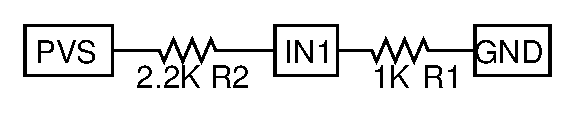
\includegraphics[height=0.8cm]{schematics/resistors}
\begin{itemize}
\item Set PVS to some voltage, read the actual value set from the message
field.
\item Click on IN1 to measure its voltage.
\item Repeat for different values of PVS. 
\item Repeat for other resistance values.
\end{itemize}

\subsection*{Observation}

The total voltage and the voltage across R1 are measured. The voltage
across R2 is $V_{PVS}-V_{R1}$. The current through R1, $I=V_{R1}/R1$.
The same amount of current flows through R2 and the voltage across
R2 can be calculated using $V_{R1}=IR1$.

\begin{tabular}{|c|c|c|c|c|}
\hline 
{\footnotesize{$V_{PVS}$}} & {\footnotesize{$V_{IN1}=V_{R1}$}} & {\footnotesize{$I=\frac{V_{IN1}}{1000}$A}} & {\footnotesize{$V_{R2}=V_{PVS}-V_{IN1}$}} & {\footnotesize{$V_{R2}=I\times2.2k$}}\tabularnewline
\hline 
\hline 
1 & .313 & .313 & .687 & .688\tabularnewline
\hline 
2 & .626 & .626 & 1.374 & 1.377\tabularnewline
\hline 
3 & .94 & .94 & 2.06 & 2.07\tabularnewline
\hline 
\end{tabular}

Expand this experiment by connecting three resistors in series and
connecting the junctions to IN1 and IN2. Another exercise is to connect
a $5.1k$ resistor from SEN to GND and measure the voltage at SEN.
Remember that SEN is internally connected to 5 volts through a $5.1k$
resistor.


\section{Calibrating Current Source\label{sec:Calibrating-Current-Source}}


\subsection*{Objective}

The actual output of constant current source may be different from
the specified 1 mA, due to the tolerance of the resistors used. It
can be measured by connecting an ammeter from CCS to GND, or by connecting
a known resistance to CCS and measuring the voltage across it. The
resistor should be in 2k to 4k range.


\subsection*{Procedure}

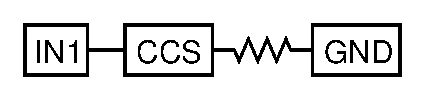
\includegraphics[height=0.8cm]{schematics/ccs-calib}
\begin{itemize}
\item Enable CCS 
\end{itemize}

\subsection*{Observation}

The measured values of the resistance is 3.876k and the voltage is
3.725 volts. The actual value of the constant current source is 3.725/3.876
= .961 mA. 

For better accuracy, the measured value should be used in experiments
using CCS.


\section{Resistances in series}


\subsection*{Objective}

Finding the effective resistance of a series combination of resistors,
$R=R1+R2+\cdots$, using a constant current source. A $560\Omega$
and a$1k\Omega$ resistors are used. 


\subsection*{Procedure}

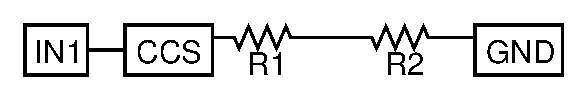
\includegraphics[height=0.8cm]{schematics/res-series}
\begin{itemize}
\item Connect R1, R2 alone and then both
\item Measure IN1 for each case
\end{itemize}

\subsection*{Observation}

\begin{tabular}{|c|c|}
\hline 
R($\Omega)$ & V(volts)\tabularnewline
\hline 
\hline 
560 & .558\tabularnewline
\hline 
1000 & 0.998\tabularnewline
\hline 
1000+560 & 1.556\tabularnewline
\hline 
\end{tabular}

Since the current is same, the total voltage drop gives the effective
resistance. It can be seen that it is the sum of the individual values,
within the measurement error. For more accurate results, use the value
of current measured as explained in section \ref{sec:Calibrating-Current-Source},
instead of 1mA.


\section{Resistances in parallel}


\subsection*{Objective}

Find the effective resistance of parallel combination of resistors,
given by $\frac{1}{R}=\frac{1}{R1}+\frac{1}{R2}+\cdots$


\subsection*{Procedure }

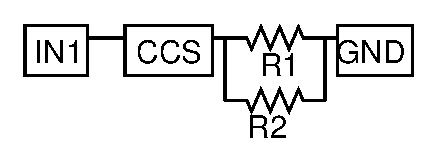
\includegraphics[height=1cm]{schematics/res-parallel}
\begin{itemize}
\item Connect 1$k\Omega$ resistor from CCS to Ground.
\item Repeat the same with two resistors connected in parallel.
\end{itemize}

\subsection*{Observation}

\begin{tabular}{|c|c|}
\hline 
$R_{connected}(\Omega)$ & $V_{measured}(V)$\tabularnewline
\hline 
\hline 
1000 & 1.008\tabularnewline
\hline 
1000$\parallel$1000 & 0.503\tabularnewline
\hline 
\end{tabular}

Since we know the current, we can calculate the resistance from the
measured voltage. As per the measured voltage the resistance of the
parallel combination is $\frac{0.503V}{0.001A}=503\Omega$.


\section{Measure resistance by comparison\label{sec:Measure-resistance-by}}


\subsection*{Objective}

Learn to apply Ohm's law to find the value of an unknown resistance
by comparing it with a known one. Voltage across a resistor is given
by $V=IR$ . If same amount of current is flowing through two different
resistors, the ratio of voltages will be the same as the ratio of
resistances, $I=\frac{V1}{R1}=\frac{V2}{R2}$.


\subsection*{Procedure }


\includegraphics[height=0.8cm]{schematics/res-compare}
\begin{itemize}
\item Connect the unknown resistor R from PVS to IN1.
\item Connect 1$k\Omega$ (R1) from IN1 to Ground.
\item Set PVS to 4 volts.
\item Measure voltage at IN1
\end{itemize}

\subsection*{Observation}

Voltage at IN1 = 1.254, implies voltage across the unknown resistor
is $4-1.254=2.746$

Current $I=\frac{1.254}{1000}=1.254mA$ . Unknown resistor value =
$\frac{2.746}{1.254mA}=2.19k\Omega$

What is the limitation of this method ? How do we choose the reference
resistor ? suppose the unknown value is in Mega Ohms, what will be
the voltage drop across a $1k\Omega$ reference resistor ? Our voltage
measurement is having a resolution of $\frac{1}{4095}$.

We will use this method later to measure the resistance of solutions,
using AC.


\section{Voltage of a lemon cell }


\subsection*{Objective}

Make a voltage source by inserting Zinc and Copper plates into a lemon.
Explore the current driving capability and internal resistance.


\subsection*{Procedure }


\subsection*{\protect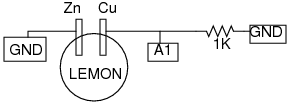
\includegraphics[height=1.3cm]{schematics/lemon-cell}}
\begin{itemize}
\item Click on A1 to measure voltage
\item Measure the voltage with and without the 1k resistor
\end{itemize}

\subsection*{Observation}

Voltage across the Copper and Zinc terminals is nearly .9 volts. Connecting
the resistor reduces it to 0.33 volts. When connected, current will
start flowing through the resistor. But why is the voltage going down
?

What is the internal resistance of the cell ?

Current is the flow of charges and it has to complete the path. That
means, current has to flow through the cell also. Depending on the
internal resistance of the cell, part of the voltage gets dropped
inside the cell itself. Does the same happen with a new dry-cell ?


\section{DC, AC and power line pickup}


\subsection*{Objective}

Introduce the concept of time dependent voltages, using a V(t) graph.
Compare the graph of DC and AC. Learn about the AC mains supply. Explore
the phenomenon of propagation of AC through free space.

\begin{figure}
\begin{centering}
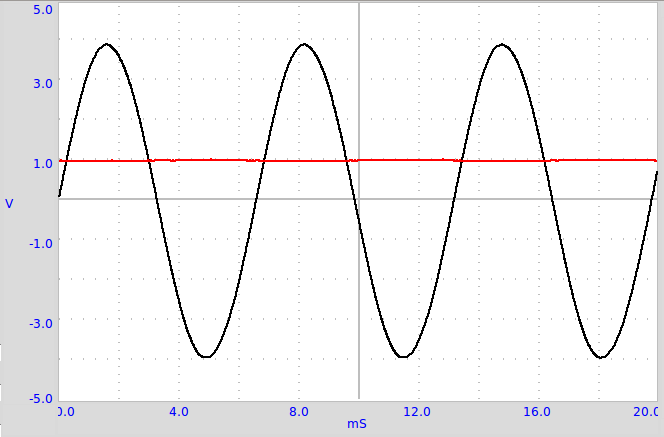
\includegraphics[width=5cm]{pics/ad-dc} 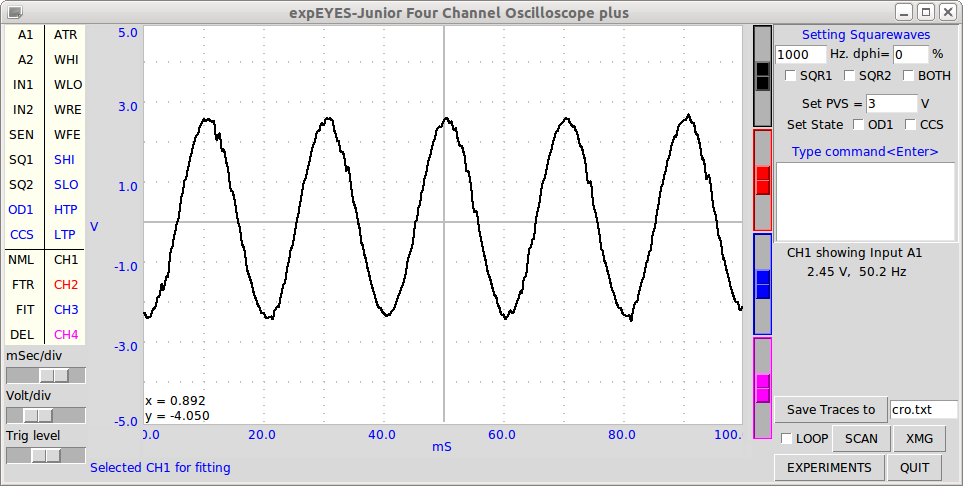
\includegraphics[width=6cm]{pics/pickup}
\par\end{centering}

\caption{Plotting Voltage Vs Time. (a) graph of DC and AC (b) AC mains pickup
\label{fig:Graph-of-DC}}
\end{figure}



\subsection*{Procedure }

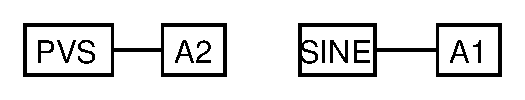
\includegraphics[height=0.7cm]{schematics/ac-dc} 
\begin{itemize}
\item Assign A1 to CH1 and A2 to CH2
\item Set PVS to 1 volt
\item Assign CH1 to FIT, to measure AC parameters.
\item Remove SINE and connect a long wire to A2
\end{itemize}
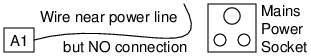
\includegraphics[height=1cm]{schematics/line-pickup}


\subsection*{Observation}

Figure \ref{fig:Graph-of-DC}(a) shows that the graph of DC is horizontal
line and for AC it changes direction and magnitude with time. The
voltage is changing with time. It goes to both negative and positive
around 150 cycles per second. This voltage waveform is generated by
using electronic circuits.

Enabling FIT option calculates the amplitude and frequency by fitting
the data with the equation $V=V_{0}\sin(2\pi ft+\theta)$ , where
$V_{0}$ is the amplitude and $f$ ~is the frequency. What is the
significance of $\theta$ in this equation ?

The power line pickup is shown in figure \ref{fig:Graph-of-DC}(b).
The frequency is obtained by fitting the data. Without making any
connection, how are we getting the AC voltage from the mains supply
?


\section{DC \& AC components of a voltage\label{sec:DC-&-AC}}


\subsection*{Objective}

Separating AC and DC components of a voltage waveform using a capacitor.

\begin{figure}
\begin{centering}
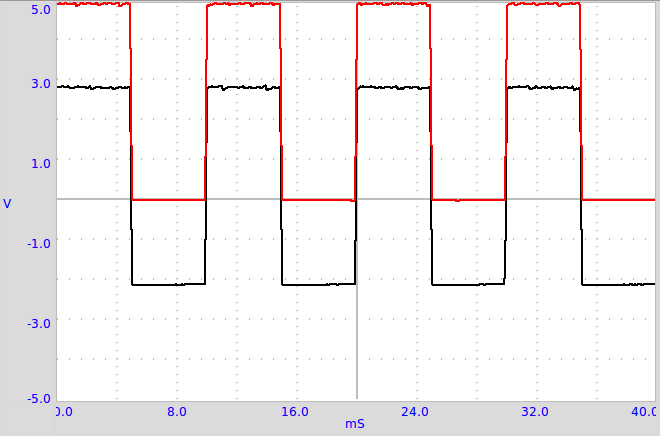
\includegraphics[width=6cm]{pics/acdc-sep-screen} 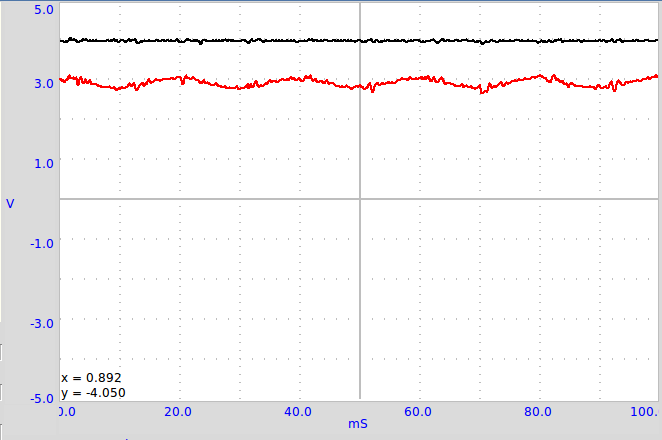
\includegraphics[width=5cm]{pics/body-resistance}
\par\end{centering}

\caption{(a) A 0 to 5V square wave, with DC component blocked (b) Resuming
electrical resistance of human body\label{fig:Square-wave}}
\end{figure}



\subsection*{Procedure }


\includegraphics[height=0.8cm]{schematics/acdc-separating}
\begin{itemize}
\item Set SQR1 to 500 Hz
\item Assign SQR1 to CH1 and A2 to CH2
\item Adjust the horizontal scale to see several cycles.
\end{itemize}

\subsection*{Observation}

The observed waveforms with and without the series capacitor are shown
in figure \ref{fig:Square-wave}. The voltage is swinging between
0 and 5 volts. After passing through the capacitor the voltage swings
from -2.5 volts to +2.5 volts.

What will you get if you subtract a 2.5 from the y-coordinate of every
point of the first graph? That is what the capacitor did. It did not
allow the DC part to pass through. This original square wave can be
considered as a 2.5V AC superimposed on a 2.5V DC.

You may need to connect a resistor from A2 to GND to see a waveform
swinging between -2.5 to +2.5 volts. Remove the resistor and observe
the result. 


\section{Resistance of human body}


\subsection*{Objective}

Get some idea about the resistance of the skin and how it varies.


\subsection*{Procedure}

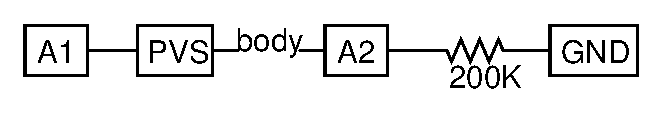
\includegraphics[height=0.8cm]{schematics/res-body}
\begin{itemize}
\item Assign A1 to CH1 and A2 to CH2
\item Join PVS and A2, through your body and measure voltage at CH2
\item Calculate your body's resistance, as given in section \ref{sec:Measure-resistance-by}
\item Repeat using SINE instead of PVS. Enable FIT to measure voltage.
\end{itemize}

\subsection*{Observation}

The observed waveform is shown in figure \ref{fig:Square-wave}(b).
Voltage at A2 is 3V, the variation is due to the 50Hz AC pickup. 


\section{Temperature dependent resistors }


\subsection*{Objective}

Show the dependence of resistance on temperature, using a thermistor,$1k\Omega@25^{0}C$,
with negative temperature coefficient. Introduce temperature sensor.


\subsection*{Procedure}

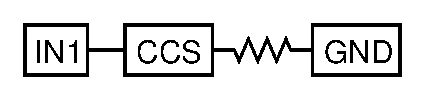
\includegraphics[height=0.8cm]{schematics/thermistor}
\begin{itemize}
\item Click on IN1 to measure the voltage
\item Repeat at different temperatures
\end{itemize}

\subsection*{Observation}

\begin{tabular}{|c|c|c|}
\hline 
Setup & V=IR & $R=\frac{V}{I}$\tabularnewline
\hline 
\hline 
In cold water & 1.2 & 1200\tabularnewline
\hline 
Room Temperature & 0.935 & 935\tabularnewline
\hline 
\end{tabular}


\section{Light dependent resistors}


\subsection*{Objective}

Learn about LDR. Measure intensity of light and its variation with
distance from the source. Use the comparison method to find out the
resistance.


\subsection*{Procedure }


\includegraphics[height=0.8cm]{schematics/ldr}
\begin{itemize}
\item Set PVS to 4V and note down the value set
\item Click on IN1 to measure it, Assign IN1 to CH1.
\item Calculate the LDR's resistance, as explained in\ref{sec:Measure-resistance-by}
\item Repeat by changing intensity of light falling on LDR
\item Connect an LED from SQR1 to GND. Set SQR1 to 10 Hz
\item Show the LED above LDR and watch waveform at IN1
\end{itemize}

\subsection*{Observation}

The resistance vary from 1k$\Omega$ to around 100 k$\Omega$ depending
on the intensity of light falling on it. The voltage is proportional
to the resistance. The resistance decreases with intensity of light.
If you use a point source of light, the resistance should increase
as the square of the distance.

Illuminate the LDR using a fluorescent tube and watch the waveform
at CH1. The frequency of the ripple is related to the mains frequency.


\section{Conductivity of water, using DC \& AC}


\subsection*{Objective}

Measure the resistance of ionic solutions, using both DC and AC voltages.
We have used normal tap water.


\subsection*{Procedure}
\begin{itemize}
\item R1 should be comparable to R, start with 10k.
\item Assign A1 to CH1 and A2 to CH2, enable FIT on both
\item Calculate the resistance as explained in section \ref{sec:Measure-resistance-by}
\item Repeat using a DC voltage, PVS instead of SINE
\end{itemize}

\subsection*{Observation}

\begin{figure}
\begin{centering}
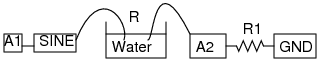
\includegraphics[width=5cm]{schematics/res-water} 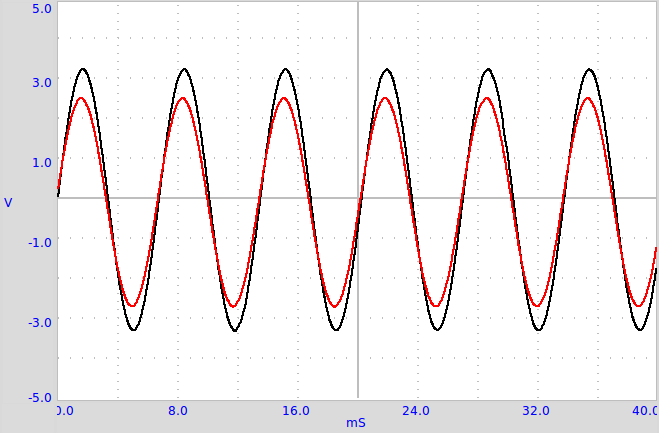
\includegraphics[width=5cm]{pics/water-conduct}
\par\end{centering}

\caption{Conductivity of water. (b)Total voltage applied and the voltage across
the 10k resistor.\label{fig:Conductivity-of-water.}}
\end{figure}


\begin{tabular}{|c|c|c|c|c|c|}
\hline 
 & $V_{total}$ & $V_{10k\Omega}$ & $V_{liq}$ & $I=\frac{V_{10k\Omega}}{1000}$ & $R_{liq}=\frac{V_{liq}}{I}$\tabularnewline
\hline 
\hline 
SINE & 3.25 & 2.6 & 0.65 & .26 mA & 2.5 k$\Omega$\tabularnewline
\hline 
PVS & 4 & 2.3 & 1.7 & .23 mA &  7.4 k$\Omega$\tabularnewline
\hline 
\end{tabular}

Observed values are shown in the table. The DC and AC resistances
seems to be very different. With DC, the resistance of the liquid
changes with time, due to electrolysis and bubble formation. The resistance
does not depend much on the distance between the electrodes, the area
of the electrode is having some effect. The resistance depends on
the ion concentration and presence of impurities in the water used.

Try changing the distance between electrodes. Try adding some common
salt and repeat the measurements. Why is the behavior different for
AC and DC ? What are the charge carriers responsible for the flow
of electricity through solutions ? Is there any chemical reaction
taking place ?


\section{Measuring Capacitance}


\subsection*{Objective}

expEYES Junior has an internal programmable current source, that can
be enabled on IN1. Connect a capacitance C and switch on current (5.5
$\mu A$) for a fixed time interval. The accumulated charge $Q=It=CV$
. By measuring $V$ , the value of C is calculated. For better results
the stray capacitance need to be subtracted. Measure C without connecting
anything to IN1, and subtract that value from the C measured with
capacitor. This method can be used for values upto 10000 pF.%
\footnote{Beyond that you need to use the Python function that can specify the
charging current, duration of charging etc.%
} Touching the capacitor during the measurement will corrupt the result. 


\subsection*{Procedure }


\includegraphics[height=0.8cm]{schematics/measure-cap}
\begin{itemize}
\item Measure C without anything connected, to get the stray capacitance.
\item connect the capacitor from IN1 to ground. 
\item Click on the Button\menuitem{Measure C on IN1}
\item Repeat with different capacitors
\end{itemize}

\subsection*{Observation}

The empty socket measures 34 pF. Several capacitors were measured.

\begin{tabular}{|c|c|}
\hline 
 Value & Measured value (pF) - 34pF\tabularnewline
\hline 
\hline 
10 & 11\tabularnewline
\hline 
20 & 19\tabularnewline
\hline 
680 & 664\tabularnewline
\hline 
180 & 176\tabularnewline
\hline 
3000 & 2900\tabularnewline
\hline 
\end{tabular}


\section{Measuring Dielectric Constant}


\subsection*{Objective}

Measure the dielectric constant of materials like glass, paper, polyester
etc., by making a capacitor. Capacitance $C=\epsilon_{0}k\frac{A}{d}$,
where $\epsilon_{0}$ is the permittivity of free space, $k$ the
dielectric constant , $A$ the overlapping area of plates and $d$
the separation between them. We have used a 13 cm x 10.6 cm piece
of window glass having 4 mm thickness to make a capacitor by pasting
metal foil on both sides.


\subsection*{Procedure }
\begin{itemize}
\item connect the capacitor from IN1 to ground. 
\item Click on the Button \menuitem{Measure C on IN1}
\item Repeat without connecting anything to IN1
\end{itemize}

\subsection*{Observation}

The measured capacitance is 225 pF. The stray capacitance is measured
after removing the wire from IN1 and it is 30pF, means C = 195pF.
$k=\frac{Cd}{\epsilon_{0}A}=\frac{195e-12\times0.004}{8.854e-12\times.13\times.106}=6.37$.
Touching the capacitor during the measurement gives wrong results. 

Using two parallel plates, the dielectric constant of liquids also
can be measured.


\section{AC Phase shift in RC circuits\label{sec:Capacitor-in-AC}}


\subsection*{Objective}

Explore the effect of a series capacitor in AC circuits, under steady
state conditions. Impedance of a Capacitor $X_{c}=\frac{1}{2\pi fC}$
, where $f$ is the frequency in Hertz and $C$ is the capacitance
in Farads. 


\subsection*{Procedure}

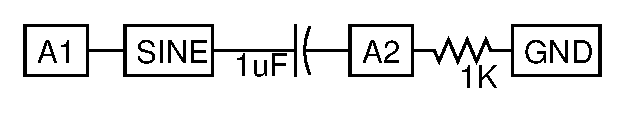
\includegraphics[height=0.8cm]{schematics/rc-acphase}
\begin{itemize}
\item Assign A1 to CH1 and A2 to CH2
\item Adjust the horizontal scale to view more than 4 cycles.
\item Right click on CH1 to calculate the phase shift.
\end{itemize}
For a detailed study select \textit{\menuitem{Study of AC Circuits}}
from \textit{\menuitem{EXPERIMENTS}.}


\subsection*{Observation}

The voltage waveform before and after the capacitor are shown in figure
\ref{fig:AC-Phase-in-RC}(a),and the calculations are shown in the
table.

\begin{tabular}{|c|c|c|c|c|}
\hline 
C(uF) & R($\Omega$) & Freq (Hz) & $\bigtriangleup\Phi$ & $\arctan\left(\frac{X_{c}}{X_{R}}\right)$\tabularnewline
\hline 
\hline 
1 & 1000 & 147.3 & 47.7 & 47.2\tabularnewline
\hline 
\end{tabular}

where $X_{c}=\frac{1}{2\pi fC}$ is the impedance of the capacitor,
Frequency is 147.3 Hz. $X_{R}$ is the resistance.

Current through a capacitor leads the voltage across it by $90^{0}$.
Why ?

Why does the phase of the voltage advance? Assume we have connected
the AC to plate A and at an instant $t=t_{0}$ the input voltage is
at zero volts. We can see that the slope of the curve is maximum there,
i.e. the rate of change of voltage is maximum. The capacitor gets
charged very fast at this point. The plate B also gathers the same
charge as plate A , that is how a capacitor works. The current to
plate B is flowing from ground through the resistor and we are measuring
the IR drop across the resistor, it will be already positive when
plate A is at zero. This results in the phase advance.
\begin{figure}
\begin{centering}
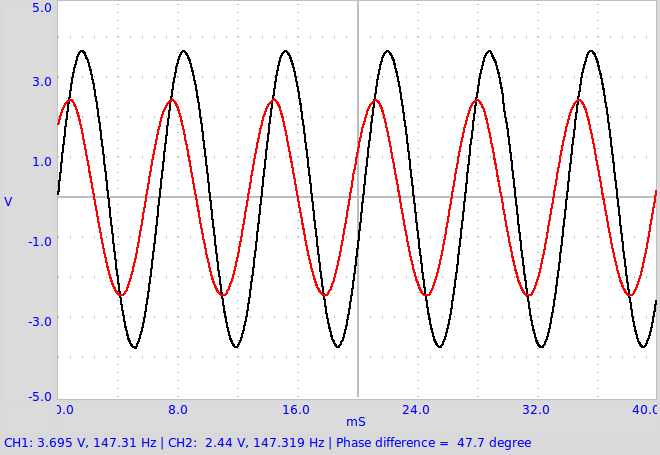
\includegraphics[width=5cm]{pics/rc-phaseshift} 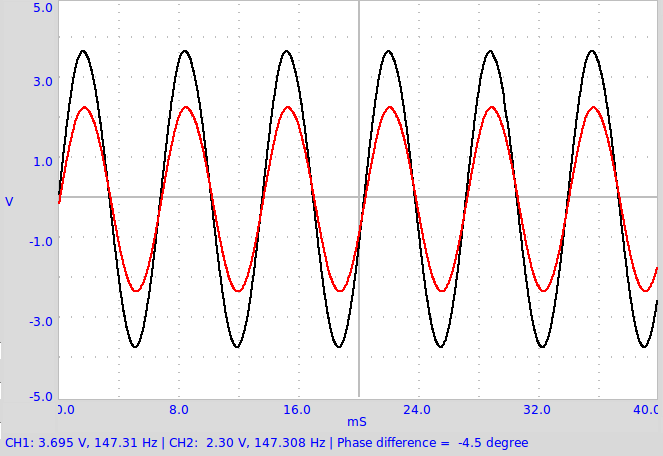
\includegraphics[width=5cm]{pics/rl-phaseshift}
\par\end{centering}

\caption{Phase shift of AC in an (a) RC circuit (b) RL circuit \label{fig:AC-Phase-in-RC}}
\end{figure}



\section{AC phase shift in RL circuits\label{sec:Inductor-in-AC}}


\subsection*{Objective}

Measure the AC voltage phase shift in an RL circuit. Impedance of
an Inductor $X_{L}=2\pi fL$ , where $f$ is the frequency in Hertz
and L is the inductance in Henry. In an LC circuit, the phase lag
across the inductor is given by the equation $\triangle\Phi=\arctan\left(\frac{X_{L}}{X_{R}}\right)$,
where R is the resistance in Ohms.


\subsection*{Procedure}


\includegraphics[height=0.8cm]{schematics/rl-acphase}
\begin{itemize}
\item Assign A1 to CH1 and A2 to CH2
\item Adjust the horizontal scale to view more than 4 cycles.
\item Right Click on A1 to view voltage, frequency and phase difference.
\end{itemize}

\subsection*{Observation}

The measured phase shifts are shown below. Waveforms for the 125 mH
inductor is shown in figure \ref{fig:AC-Phase-in-RC}(b). The resistance
of the inductor also should be included while calculating the phase
shift.%
\footnote{http://www.play-hookey.com/ac\_theory/ac\_inductors.html%
}.

\begin{tabular}{|c|c|c|c|}
\hline 
L(mH) & $R=R_{coil}+R_{ext}$($\Omega$) & $\bigtriangleup\Phi=\arctan\left(\frac{X_{L}}{X_{R}}\right)$ & $\bigtriangleup\Phi_{measured}$\tabularnewline
\hline 
\hline 
125 & 565 + 560 & 3.71 & -3.8\tabularnewline
\hline 
\end{tabular}

Insert an iron or ferrite core to the coil and observe the effect
of ferromagnetic materials. Self Inductance of a solenoid is given
by $L=\frac{\mu N^{2}A}{l}$ , where N is the number of turns, A is
the cross sectional area, $\mu$ is the permeability of the surrounding
media and $l$ is the length.


\section{Transient Response of RC circuits\label{sec:Capacitor-charging-&}}


\subsection*{Objective}

Plot the voltage across a capacitor, when it is charged by applying
a voltage step through a resistor. Calculate the value of the capacitance
from the graph.


\subsection*{Procedure}


\includegraphics[height=0.8cm]{schematics/RCcircuit} 
\begin{itemize}
\item From \textit{\menuitem{EXPERIMENTS}} , select \textit{\menuitem{RC Circuit}} 
\item Click on \textit{0->5V STEP} and \textit{5->0V step} Buttons to plot
the graphs
\item Adjust the horizontal scale, if required, and repeat.
\item Calculate RC time constant.
\item Use CCS instead of OD1 to charge capacitor with constant current.
\end{itemize}

\subsection*{Observation}

\begin{figure}
\begin{centering}
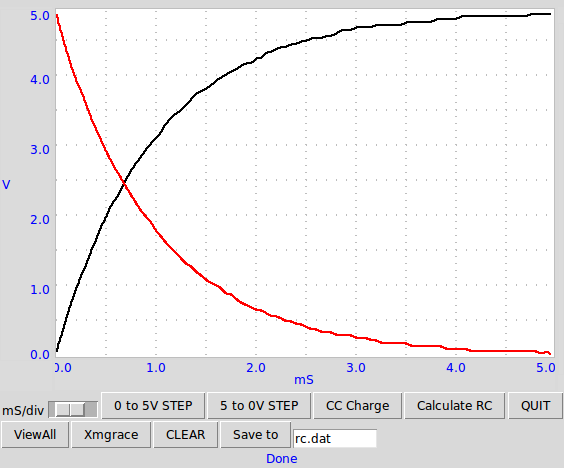
\includegraphics[width=5cm]{pics/RC-curves} 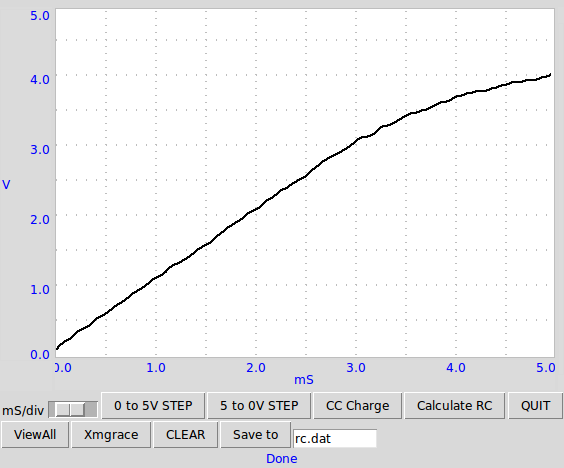
\includegraphics[width=5cm]{pics/cap-linear}
\par\end{centering}

\caption{(a)Transient response of RC circuit. (b) Charging of capacitor with
constant current. \label{fig:Transient-RC}}
\end{figure}


Applying a 0 to 5V step makes the voltage across the capacitor to
rise exponentially as shown in the figure\ref{fig:Transient-RC}(a).
By fitting the discharge curve with $V(t)=V_{0}e^{-\frac{t}{RC}}$
,we can extract the RC time constant and find the values of capacitance
from it. 

The voltage across a capacitor is exponential only when it is charged
trough a linear element, a resistor for example. When charged from
a constant current source, the voltage shows linear increase, as shown
in figure \ref{fig:Transient-RC}(b), because $Q=It=CV$ , and voltage
increases linearly with time as $V=\left(\frac{I}{C}\right)t$ .


\section{Transient Response of RL circuits}


\subsection*{Objective}

Explore the nature of current and voltage when a voltage step is applied
to resistor and inductor in series. By measuring the voltage across
the inductor as a function of time, we can calculate its inductance.

In an RL circuit $V=IR+L\frac{dI}{dt}$ and solving this will give
$I=I_{0}e^{-\frac{R}{L}t}$. The coefficient of the exponential term
R/L can be extracted from the graph of voltage across the inductor.
The resistance of the inductor coil should be included in the calculations,
$R=R_{ext}+R_{L}$. %
\footnote{http://nptel.iitm.ac.in/courses/Webcourse-contents/IIT-KANPUR/esc102/node14.html%
}


\subsection*{Procedure}


\includegraphics[height=0.8cm]{schematics/RLcircuit}
\begin{itemize}
\item Inductor is the 3000 Turn coil
\item From \textit{\menuitem{EXPERIMENTS}} select \textit{\menuitem{RL Circuit}}
\item Click on \textit{0->5V STEP} and \textit{5->0V step} Buttons to plot
the graphs
\item Adjust the horizontal scale, if required, and repeat.
\item Calculate the value of inductance
\item Insert an iron core into the inductor and repeat
\end{itemize}

\subsection*{Observation}

\begin{figure}
\begin{centering}
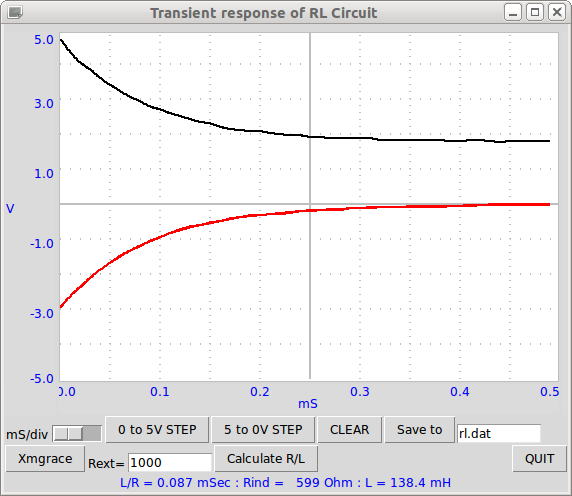
\includegraphics[width=5cm]{pics/RL-curves}
\par\end{centering}

\caption{Transient response of RL circuit\label{fig:Transient-RL}}
\end{figure}


The transient response of the inductor is shown in figure \ref{fig:Transient-RC}.
The exponential curve is fitted to extract the L/R value. The resistance
of the coil is measured by comparing it with the known external resistance
under DC conditions. IN1 is connected to OD1 for a more accurate measurement
of the coil resistance.

The applied voltages are above zero, but the graph went to negative
voltages. Why ?

What was the current before doing the 5->0 step ? What is back EMF
?

Repeat with two coils in series, by (a) placing them far away (b)
placing one over the other and (c) after changing the orientation.
The effect of mutual inductance can be seen.


\section{Transient response of LCR circuits\label{sec:Step-Response-ofRLC}}


\subsection*{Objective}

Explore the oscillatory nature of L and C in series. Resonant frequency
of series LC circuit is given by $\omega_{0}=\frac{1}{2\pi\sqrt{LC}}$.
The damping factor is $\frac{R}{2}\sqrt{\frac{C}{L}}$, and it is
equal to 1 for critical damping.%
\footnote{http://en.wikiversity.org/wiki/RLC\_circuit%
} Depending upon the value of C/L and R, the response could be under-damped,
critically-damped or over-damped. 

\begin{figure}
\begin{centering}
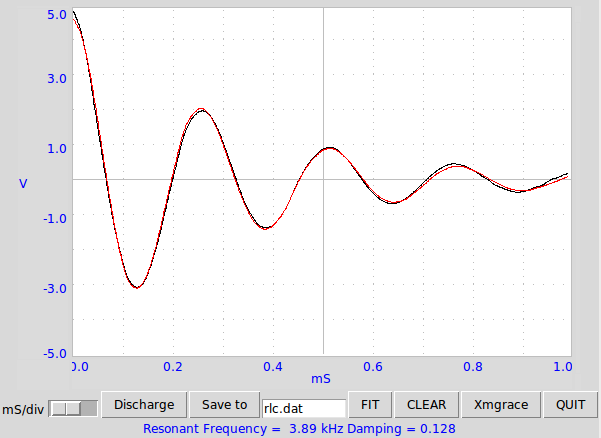
\includegraphics[width=5cm]{pics/RLC-curves} 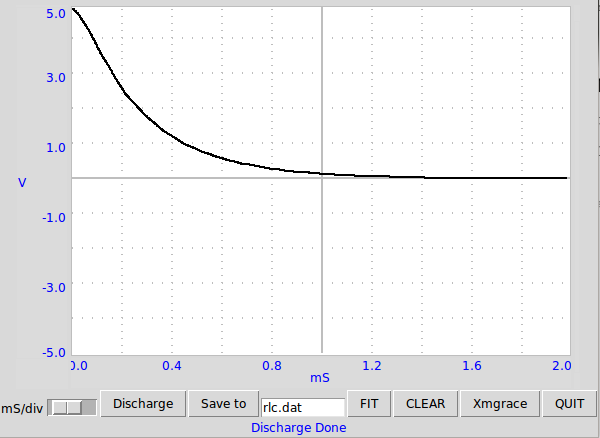
\includegraphics[width=5cm]{pics/RLC-curve-damped}
\par\end{centering}

\caption{Transient response of LCR circuit,(a)Under-damped (b)Over-damped.\label{fig:LCR Transient-response}}
\end{figure}



\subsection*{Procedure }


\includegraphics[height=0.8cm]{schematics/LCRcircuit} 
\includegraphics[height=0.7cm]{schematics/LCRRcircuit}
\begin{itemize}
\item From \textit{\menuitem{EXPERIMENTS}} select\textit{ \menuitem{RLC Discharge}} 
\item Click on 5->0V STEP. Adjust x-axis and repeat if required.
\item FIT the graph to find the resonant frequency \& Damping.
\item Repeat the experiment with different values of L, C and R
\item Repeat with a resistor in series.
\end{itemize}

\subsection*{Observation}

We have used the 3000 turn coil and a 0.1uF capacitor, added a 2.2k
series resistor in the second case. The voltage across the capacitor
after a 5 to 0V step is shown in figure \ref{fig:LCR Transient-response}
.The measured resonant frequency tallies with $f=\frac{1}{2\pi}\sqrt{\frac{1}{LC}}$
, within the component tolerance values.


\section{RC Integration \& Differentiation }


\subsection*{Objective}

RC circuits can integrate or differentiate a voltage waveform with
respect to time. A square wave is integrated to get a triangular wave
and differentiated to get spikes at the transitions.


\subsection*{Procedure}


\includegraphics[height=0.8cm]{schematics/rc-integ} 
\begin{itemize}
\item Set SQR2 to 1000Hz
\item Assign SQR2 to CH1 and A1 to CH2
\item Adjust the horizontal scale to view more than 4 cycles.
\item Set SQR2 to 1kHz (T = 1mS) and other values and view the waveforms.
\item Repeat the same for RC differentiator, at 100Hz.
\end{itemize}

\includegraphics[height=0.8cm]{schematics/rc-diff}


\subsection*{Observation}

\begin{figure}
\begin{centering}
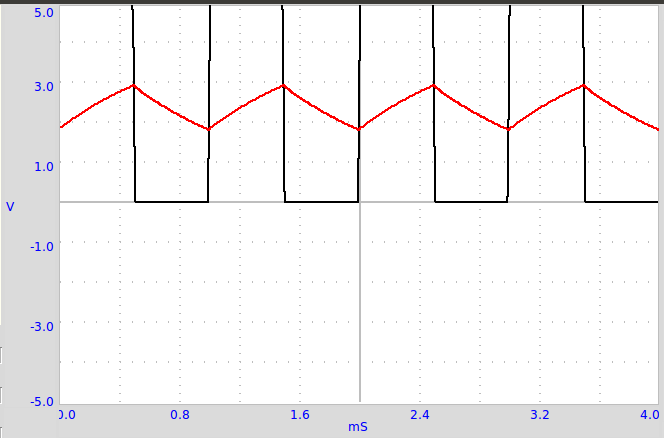
\includegraphics[width=5cm]{pics/rc-integ1khz}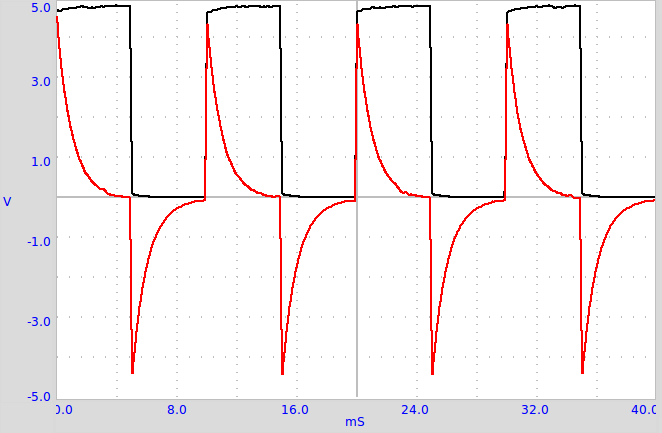
\includegraphics[width=5cm]{pics/rc-diff100Hz}
\par\end{centering}

\caption{(a)1kHz Squarewave after RC Integrator (b) 100Hz after RC Differentiator\label{fig:RC-int-diff}}
\end{figure}


Integration observed at 1kHz and differentiation at 100Hz are shown
in figure \ref{fig:RC-int-diff}, using an RC value of 1 milliseconds.
When the time period becomes comparable with the RC value, the output
waveform is triangular. The differentiation can only be shown at lower
frequency since capturing the narrow spike requires a fast oscilloscope.


\section{Fourier Analysis\label{sec:Fourier-Transform-**}}


\subsection*{Objective}

Learn about Fourier Transform of a signal. Time and Frequency domain
representations.


\subsection*{Procedure}

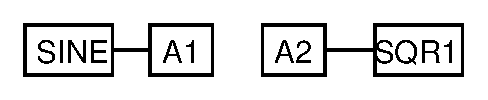
\includegraphics[height=0.8cm]{schematics/ftran}
\begin{itemize}
\item Set SQR1 to 150Hz
\item Assign A1 to CH1 and SQR1 to CH2
\item Assign CH1 \& CH2 to FT to view the Fourier transform
\end{itemize}

\subsection*{Observation}

\begin{figure}
\begin{centering}
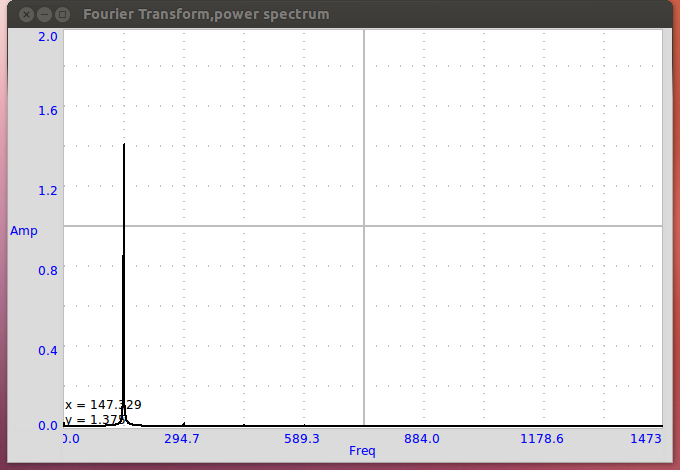
\includegraphics[width=5cm]{pics/fft-sine147Hz} 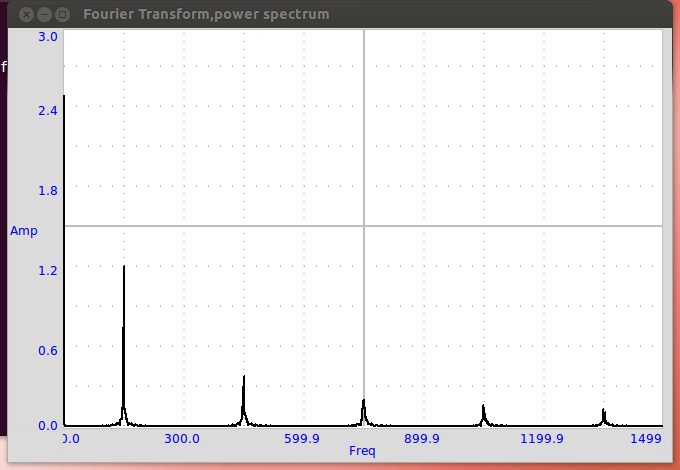
\includegraphics[width=5cm]{pics/fft-sqr150Hz}
\par\end{centering}

\caption{Frequency spectrum of (a)Sine wave. (b) Squarewave\label{fig:Frequency-spectrum-of}}
\end{figure}


In the Fourier transform plot, frequency is on the x-axis and the
y-axis shows the relative strength of each frequency components of
the signal. This is called the frequency domain representation%
\footnote{http://en.wikipedia.org/wiki/Fourier\_transform%
}. For the sine wave there is only one dominant peak, the smaller ones
are a measure of distortion of the sine wave. 

A square wave function can be represented as $f(\theta)=sin(\theta)+\frac{sin(3\theta)}{3}+\frac{sin(5\theta)}{5}+\cdots$.
In the Fourier transform of a square wave of frequency $f$ , there
will be a $3f$ component (having an amplitude of one third of $f$
), $5f$ component (amplitude one fifth) etc. as shown in the figure
\ref{fig:Frequency-spectrum-of}(b). Note the peak at 0 Hz, due to
the DC component.


\end{document}
